% Figure 4 -- Diagnostic Accuracy Comparison (pgfplots bar chart)
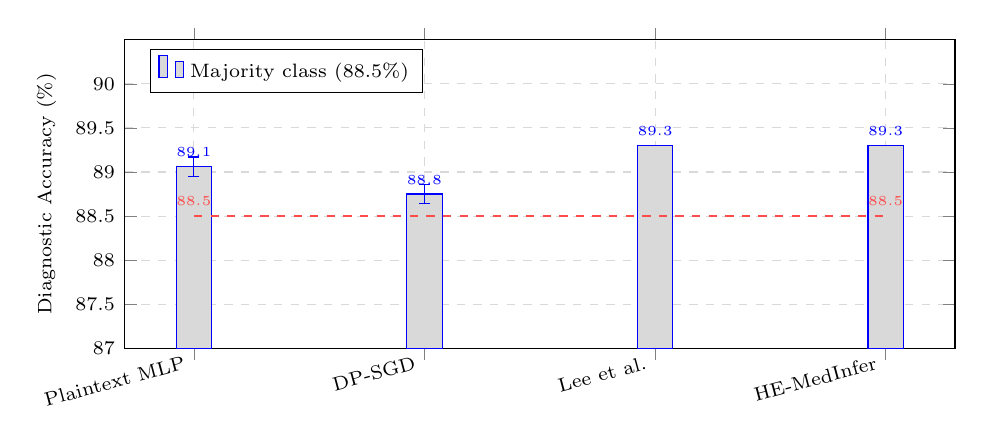
\begin{tikzpicture}
\begin{axis}[
  ybar,
  width=\columnwidth,
  height=5.5cm,
  bar width=0.45cm,
  ymin=87, ymax=90.5,
  ylabel={Diagnostic Accuracy (\%)},
  symbolic x coords={Plaintext MLP, DP-SGD, Lee et al., HE-MedInfer},
  xtick=data,
  x tick label style={font=\scriptsize, rotate=15, anchor=east},
  ytick={87,87.5,88,88.5,89,89.5,90},
  yticklabel style={font=\scriptsize},
  ylabel style={font=\scriptsize},
  nodes near coords,
  nodes near coords style={font=\tiny, /pgf/number format/.cd, fixed, precision=1},
  error bars/y dir=both,
  error bars/y explicit,
  legend pos=north west,
  legend style={font=\scriptsize},
  grid=major,
  grid style={dashed, gray!30},
]
% Error bars are 95% CI half-widths (t-distribution, df=9) computed from the
% 10 real per-seed accuracy values in results/plaintext.json and
% results/dpsgd.json; Lee et al. (proxy) and HE-MedInfer are single real
% runs with no replication, so no CI can be computed without fabrication --
% they are plotted with zero-width bars, per the caption's disclosure.
\addplot+[fill=gray!30, error bars/.cd, y dir=both, y explicit]
  coordinates {
    (Plaintext MLP,  89.06) +- (0,0.11)
    (DP-SGD,         88.75) +- (0,0.11)
    (Lee et al.,     89.3) +- (0,0)
    (HE-MedInfer,    89.3) +- (0,0)
  };
% Majority-class baseline: 88.5% (11.5% outcome prevalence)
\addplot[red!70, dashed, thick, sharp plot, update limits=false]
  coordinates {(Plaintext MLP,88.5) (HE-MedInfer,88.5)};
\addlegendentry{Majority class (88.5\%)}
\end{axis}
\end{tikzpicture}
